\documentclass{scrartcl}
\usepackage[utf8]{inputenc}
\usepackage{version}
\usepackage{hyperref} \begin{comment} links \end{comment}
\usepackage{amsfonts} \begin{comment} mathbb \end{comment}
\usepackage{graphicx} \begin{comment} images \end{comment}
\usepackage{subfig} \begin{comment} subfigure \end{comment}
\usepackage{algorithm}
\usepackage{algpseudocode} \begin{comment} pseudocode \end{comment}

\usepackage[
backend=bibtex,
style=alphabetic,
sorting=ynt
]{biblatex}
\addbibresource{refs.bib}

\AtEndDocument{\printbibliography}

\title{Forest Cover type Classification}
\subtitle{Project of Statistical methods for machine learning}
\author{Sara Ramazzotti - 960893 - \href{mailto:sara.ramazzotti@studenti.unimi.it}
{sara.ramazzotti@studenti.unimi.it}}
\date{A.Y. 2020-21}

\begin{document}

\maketitle

\textit{I declare that this material, which I now submit for assessment, is entirely my own work and has not been taken from the work of others, save and to the extent that such work has been cited and acknowledged within the text of my work. I understand that plagiarism, collusion, and copying are grave and serious offences in the university and accept the penalties that would be imposed should I engage in plagiarism, collusion or copying. This assignment, or any part of it, has not been previously submitted by me or any other person for assessment on this or any other course of study.}

\section{Assignment}
Download the Cover Type Dataset \cite{fctd} for multiclass classification. Implement AdaBoost from scratch and run it using decision stumps (binary classification rules based on single features) as base classifiers to train seven binary classifiers, one for each of the seven classes (one-vs-all encoding). Use external cross-validation to evaluate the multiclass classification performance (zero-one loss) for different values of the number T of AdaBoost rounds. In order to use the seven binary classifiers to make multiclass predictions, use the fact that binary classifiers trained by AdaBoost have the form $ h(x)=sgn(g(x)) $ and predict using $ argmax_{i}g_{i}(x) $ where $ g(x) $ corresponds to the binary classifier for class \textit{i}.

\section{Introduction}

\subsection{Analysis of the dataset}
The \textit{Forest Cover Type Dataset} presents the observations collected from each landmark of the Roosevelt National Forest in Colorado. It has 55 columns, where the first 54 are the features of the land considered and the last one indicates the preferred \textit{cover type}. It presents 581012 samples \cite{fctd}.
Data from the first ten columns are numerical values $ \in \mathbb{Z} $ ; the remaining represents binary features $ \in \{0, 1\}$.

The last column, as said, indicates the expected cover type classification. There are seven type of covers and they are indicated as numbers in the set $\{1, 2, 3, 4, 5, 6, 7\}$. It has to be noticed that the dataset is not balanced, for each class there are different numbers of samples. We can see the distribution of the labels in the following histogram: 
\begin{figure}[h!]
  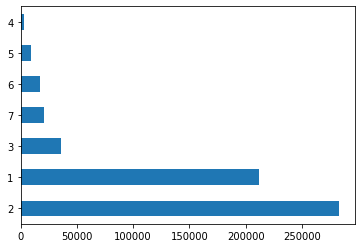
\includegraphics[width=0.5\textwidth]{imgs/cover_type_distribution.png}
  \centering
  \caption{Cover type distribution. On the ordinate axis there are the seven classes, in ascending order w.r.t. the number of samples on the abscissa axis.}
  \label{figure:distribution}
\end{figure}

Luckily the raw data does not present null values, so the dataset does not need manipulation. The distribution of each feature can be found at \href{https://www.kaggle.com/uciml/forest-cover-type-dataset}{Kaggle's page}.

\subsection{Adaboost approach}
\subsubsection{Week learners used}
Adaboost is an ensemble method used to achieve a bias-variance tradeoff better than the one achieved by the single combined predictors that are used by the algorithm. Adaboost can train very simple weak learners, such as decision stumps. Decision stumps are classifiers of the form $h_i,_\tau : \mathbb{R}^d \to \{-1,1\}$ defined by $h_i,_\tau = sgn(x_i - \tau) \cdot b$, where $i=1...d$, $\tau \in \mathbb{R}$ and $b\in{-1,1}$. In the implementation $b$ is chosen as +1 for simplicity \cite{boosting-notes}. Note that \textit{d} is the number of features of the samples, in our case 54, and $\tau$ is the number that permits to split the samples in two groups: one labeled with +1 and the other with -1. Obviously the labels predicted in such a way are not perfectly labeled, but we can chose $\tau$ and $i$ in order to pick in the set of all possible couples of $(i, \tau)$ the one that generates the predictor with the minimum weighted training error (ERMDS \cite{ermds}). This approach permits to include in the train phase a weight distribution of the samples, useful for Adaboost.

\subsubsection{Multiclass classification}
The base version of Adaboost is designed for binary classification. As previously mentioned, our dataset presents seven different classes. A way to apply Adaboost with decision stumps on this dataset is to train seven different adaboost classifiers and then combine the results using $ argmax_{i}g_{i}(x) $ to predict the labels, where $ g(x) $ corresponds to the binary classifier for class \textit{i}. Each predictor is trained with the dataset modified using the encoding \textit{one-vs-all}: i.e. for class \textit{2} we mark as +1 the samples classified as 2, and as -1 the samples classified as 1, 3, 4, 5, 6 or 7. In such a way each predictor tries to predict if the example belongs to that particular class or to another one. Moreover, doing this kind of approach it can be studied the behaviour of adaboost for each type of sample. The idea is that maybe it is easier to classify some classes with respect to others and the class that is predicted with more difficulty could affect the entire multiclass prediction.

At this point I can present the pseudocode of the approach adopted. I need to feed into the model the entire training set untouched. Then the fit phase maps the given set to the form one-vs-all one class at a time. For each training set mapped this way, the classic adaboost can be executed. At the end of the train phase, for each class the model will have memorized the weak predictors trained at each round of the algorithm, their weights and their errors (useful for the analysis). These groups of predictors-weights are then used to form the seven binary classifiers of our interest, in the form $f = sgn(\sum_{n=1}^{T} w_i h_i) $. Finally they are grouped together to get the multiclass prediction: $ argmax_{i}f_{i} $.

\begin{algorithm}
\caption{Pseudocode of the multiclassifier Adaboost}\label{alg:cap}
\begin{algorithmic}
\State $binaryPredictors \gets [ ]$
\For{$k$ in classes}
    \State $dataset \gets map(dataset, k)$
    \State $predictor \gets adaboost(dataset, T)$
    \State  add predictor to binaryPredictors
\EndFor
\State \Return predict with $ argmax_{i}binaryPredictors_{i}$
\end{algorithmic}
\end{algorithm}

\section{Analysis of the output}
In this section I want to show the results of the cross validation on my implementation of Adaboost. The cross validation was made on 5 folds, using the implementation of KFold from \textit{scikit learn} \cite{kfold}. 
The main goal was the evaluation of the algorithm at the increasing of rounds of adaboost. For better timing performance two decisions were made:
\begin{itemize}
\item first of all, the python notebook that execute the cross validation was runned with google colab;
\item secondly, two experiments were made using two subsamples of the entire dataset.
\end{itemize}

The first subsample considered is built with a random draw of one thousand examples from the original dataset. This small group of data permits to run the cross validation more quickly, to use a quite large number of rounds (35 is the chosen number) and to better understand the trend of the errors. It can be seen in the top-left subfigure of Fig.~\ref{figure:errors_1000} that the algorithm does not behave so bad and that the errors tend to decrease even if not so quickly apparently.

As we know from the theory \cite{boosting-notes} the training error of adaboost is upper bounded by $exp(-2\sum_{i=1}^{T} \gamma_i^2)$ where $\gamma_i = 0.5-\epsilon_i$ and $\epsilon_i$ is the weighted training error of the weak learner of round i. So the training error should go down exponentially with respect to T. I can verify this saving the errors of the weak classifiers. In Fig.~\ref{figure:tab1_ub_1000} and ~\ref{figure:tab2_ub_1000} are represented in the first column the upper bounds and the training error for each single class considered, and in the second column the trend of the errors $\epsilon_i$. Those results are taken from the last fold that have fitted the model. As you can see the trend of the training errors tends to be under the upper bound at every class and in particular 0 is reached by the class 4, around the 18th round. Even classes 3, 5, 6, and 7 almost reach the zeros. Instead classes 1 and 2 have the zeros quite far from their actual error state. We can see in the graphs of Fig.~\ref{figure:errors_1000} the results of the cross validation for each one-vs-all study, which confirms the trends just discussed. For cover types 1 and 2 the errors goes down not so quickly, as expected. A possible reason of these facts is that there are not sufficient data to discriminate the two more present groups of the dataset (recall Fig.~\ref{figure:distribution}) with respect to the other four or between them. Beside class 4 for which the zero is reached, in the other classes even if it is not clear looking at the lines that the errors are reaching the zero, it can be seen in the ordinate axis that the errors are really small and quite near the zero. Moreover the test errors too are really low so for our dataset the data characterizing the samples of the classes with less samples are really well used by our stumps.

The second group of data considered has a grater number of samples, one hundred thousand. Applying cross validation on this set is much more expensive in terms of time complexity so I reduced the number of rounds assessed. We know that this implementation of adaboost is efficient, because the fitting time of the decision stump is efficient in the order of $\mathcal{O}(md)$ where $d$ is the number of features (54) and $m$ the number of examples. Though this process is efficient it has to be noticed that if $m$ is a big number it still takes a lot of time, considering that we need to train a different weak learner at every round of adaboost and that in this particular implementation we need seven of them. Moreover during the cross validation we need to repeat the process for every training group. 

The results do not differ too much from those of the previous experiment. It confirms the hypothesis of some underling schema of the observations that tend to make difficult the recognition of classes 1 and 2 alone as can be seen in Fig.~\ref{figure:tab1big}. On the other hand It can be noticed in graphs of Fig.~\ref{figure:errors_big} that with this group the difference between test and training errors is even closer than the previous observation, which means that the characteristics of the test and train sets considered in CV are reasonably quite the same.

\begin{figure}
\centering
{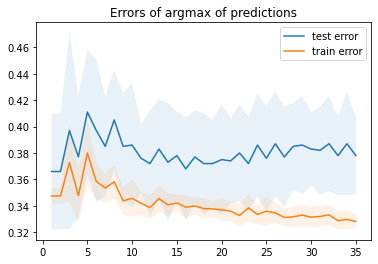
\includegraphics[width=.45\textwidth]{imgs/N1000_T35/full_plot_1000.png}} \quad
{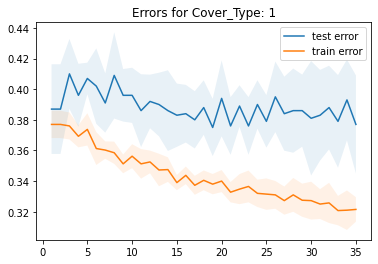
\includegraphics[width=.45\textwidth]{imgs/N1000_T35/cv_1_1000.png}} \\
{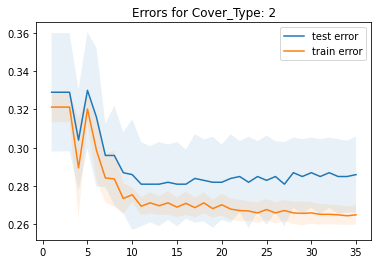
\includegraphics[width=.45\textwidth]{imgs/N1000_T35/cv_2_1000.png}} \quad
{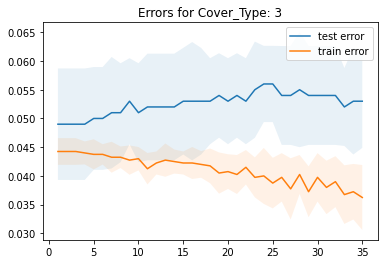
\includegraphics[width=.45\textwidth]{imgs/N1000_T35/cv_3_1000.png}} \\
{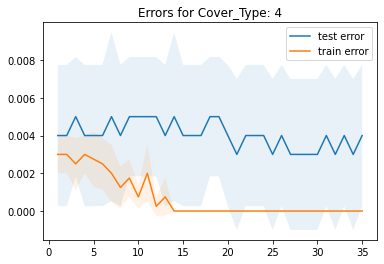
\includegraphics[width=.45\textwidth]{imgs/N1000_T35/cv_4_1000.png}} \quad
{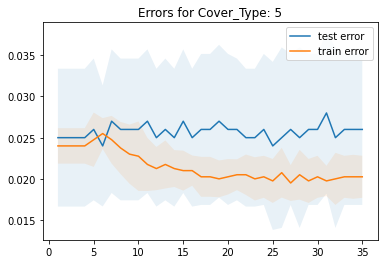
\includegraphics[width=.45\textwidth]{imgs/N1000_T35/cv_5_1000.png}} \\
{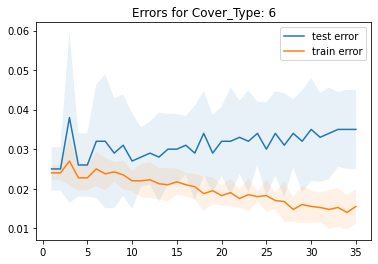
\includegraphics[width=.45\textwidth]{imgs/N1000_T35/cv_6_1000.png}} \quad
{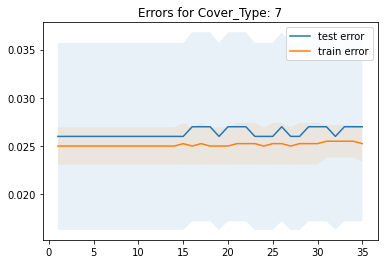
\includegraphics[width=.45\textwidth]{imgs/N1000_T35/cv_7_1000.png}}
\caption{Results of CV on the set of 1000 examples. Means of Training and Test errors at the different stage of T. In the top-left subfigure is represented the true resulting classification and in the others subfigures it can be seen the error of the single class classification. Areas with a shaded color indicate the standard deviation at that point.}
\label{figure:errors_1000}
\end{figure}

\begin{figure}
  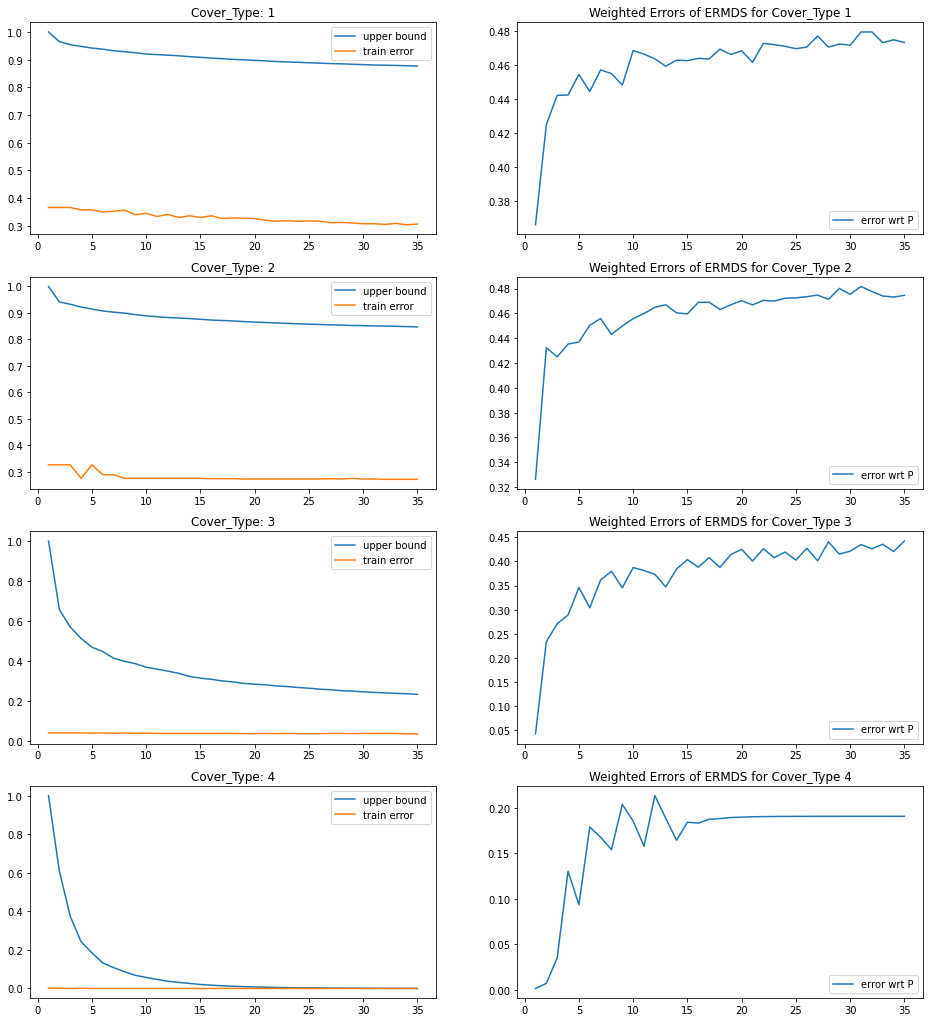
\includegraphics[width=1\textwidth]{imgs/N1000_T35/upper_bound_1000_pt1.png}
  \centering
  \caption{How the chosen weak learners for the last fold behave with respect to training error. Sample of 1000 examples.}
  \label{figure:tab1_ub_1000}
\end{figure}
\begin{figure}
  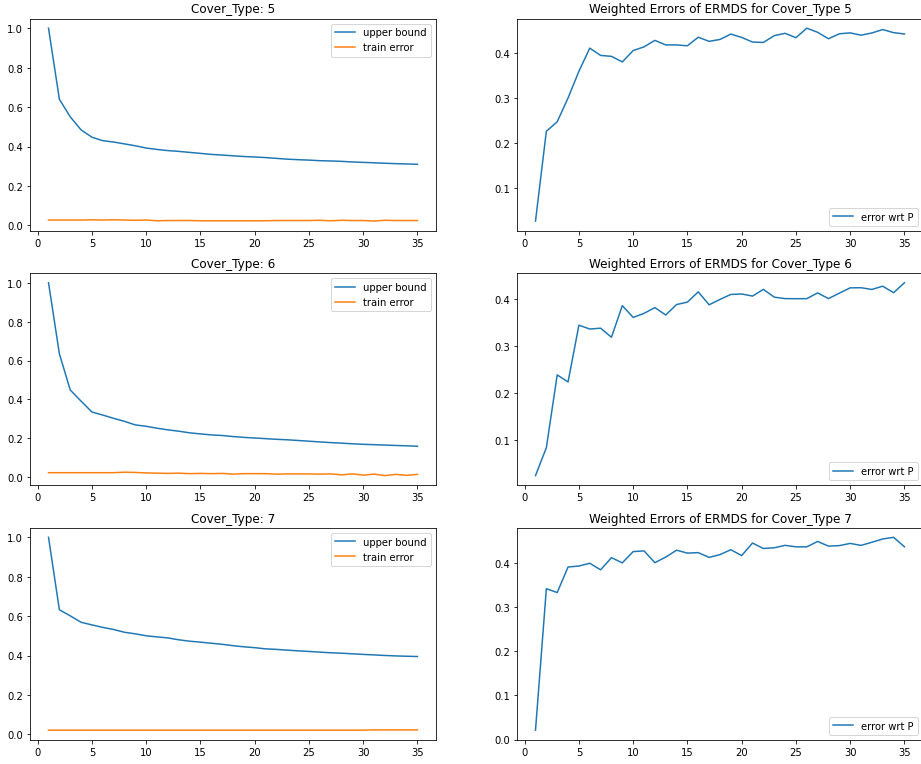
\includegraphics[width=1\textwidth]{imgs/N1000_T35/upper_bound_1000_pt2.png}
  \centering
  \caption{Cont. Fig.~\ref{figure:tab1_ub_1000}}
  \label{figure:tab2_ub_1000}
\end{figure}

\begin{figure}
\centering
{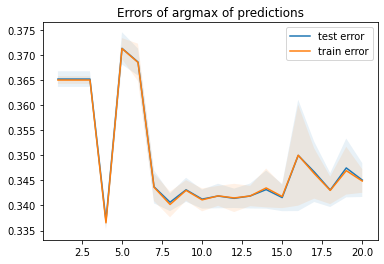
\includegraphics[width=.45\textwidth]{imgs/N100000_T20/full_plot_big.png}} \quad
{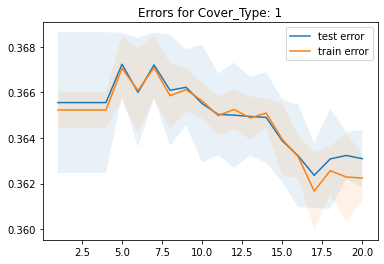
\includegraphics[width=.45\textwidth]{imgs/N100000_T20/cv_1_big.png}} \\
{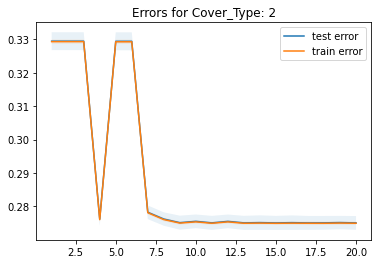
\includegraphics[width=.45\textwidth]{imgs/N100000_T20/cv_2_big.png}} \quad
{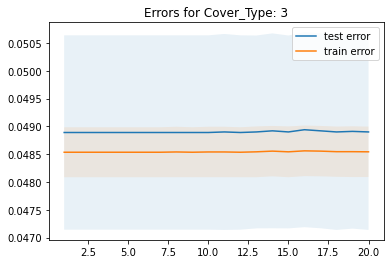
\includegraphics[width=.45\textwidth]{imgs/N100000_T20/cv_3_big.png}} \\
{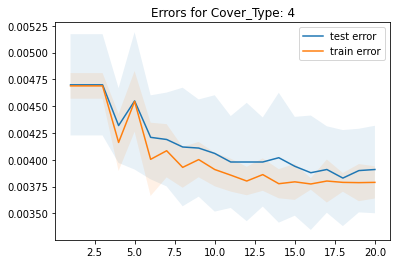
\includegraphics[width=.45\textwidth]{imgs/N100000_T20/cv_4_big.png}} \quad
{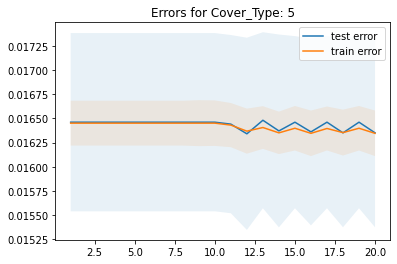
\includegraphics[width=.45\textwidth]{imgs/N100000_T20/cv_5_big.png}} \\
{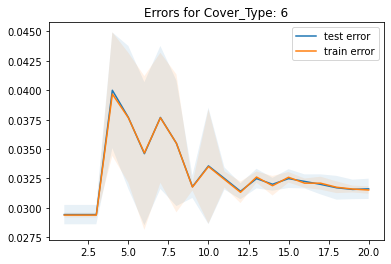
\includegraphics[width=.45\textwidth]{imgs/N100000_T20/cv_6_big.png}} \quad
{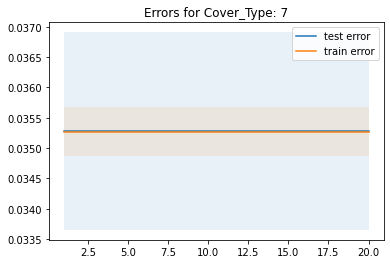
\includegraphics[width=.45\textwidth]{imgs/N100000_T20/cv_7_big.png}}
\caption{Same description as Fig.~\ref{figure:errors_1000} for the bigger dataset.}
\label{figure:errors_big}
\end{figure}

\begin{figure}
  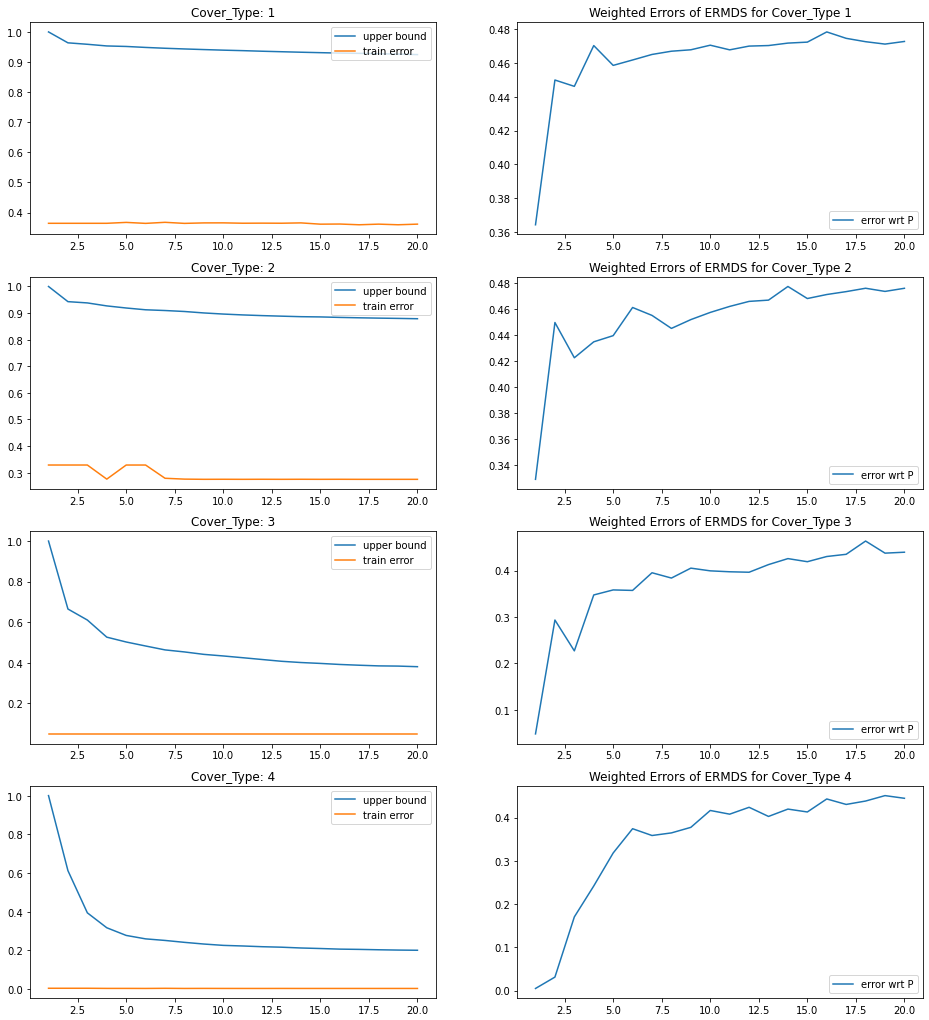
\includegraphics[width=1\textwidth]{imgs/N100000_T20/upper_bound_big_pt1.png}
  \centering
  \caption{Same description as Fig.~\ref{figure:tab1_ub_1000} for the bigger dataset.}
  \label{figure:tab1big}
\end{figure}
\begin{figure}
  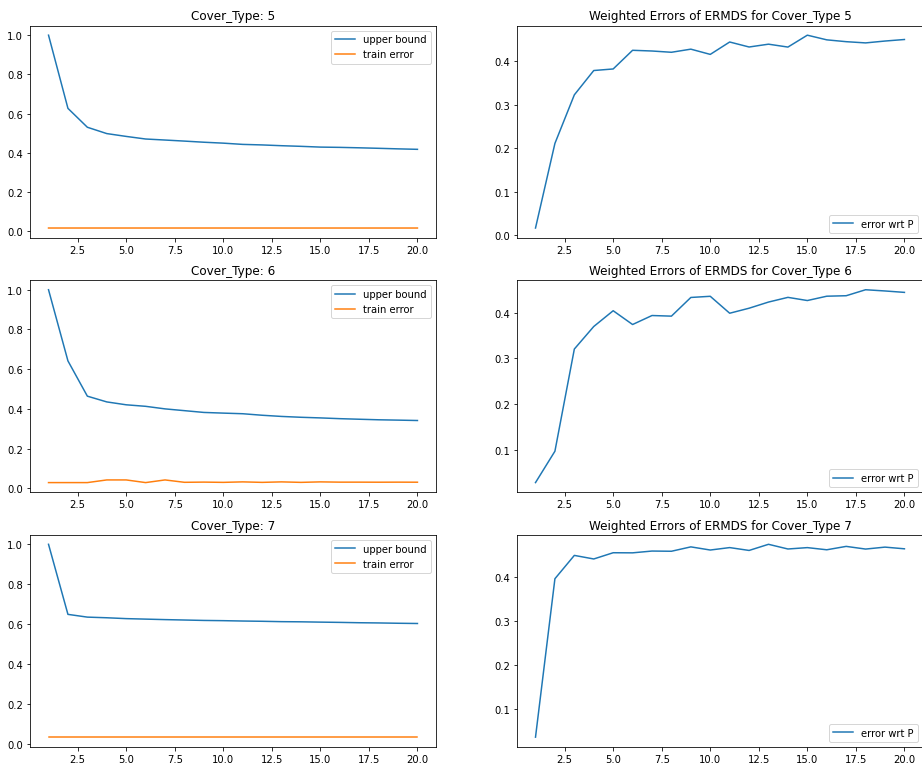
\includegraphics[width=1\textwidth]{imgs/N100000_T20/upper_bound_big_pt2.png}
  \centering
  \caption{Cont. Fig.~\ref{figure:tab1big}}
  \label{figure:tab2big}
\end{figure}

\section{Conclusions}

In this study the implementation follows a naive approach to multiclassification, exploiting the fact that the binary predictors are of the form sgn and that when they are combined they can predict by majority the true label.
Another approach, which would have speeded up the analysis, is to use an adaboost algorithm specifically studied for multiclassification \cite{multi-adaboost}.

\newpage

\end{document}
